\documentclass[./../SoftwareEngineering.tex]{subfiles}

\section{Design Concepts}
Tập hợp các khái niệm (concept) thiết kế phần mềm cơ bản đều được triển khai khắp chiều dài lịch sử thiết kế phần mềm. Mặc dù mức độ phổ dụng của các phần mềm thay đổi qua từng năm, nhưng mỗi loại trong chúng đều có thể đứng vững trước thử thách của thời gian. Mỗi người lại cung cấp thiết kế với một nền móng đến từ nhiều phương pháp thiết kế phức tạp. Chúng có thể giúp bạn trả lời theo những câu hỏi dưới đây:
\begin{itemize}
	\item Các tiêu chuẩn để chia phần mềm thành các thành phần riêng lẻ??
	\item Làm thế nào để các hàm hoặc cấu trúc dữ liệu được phân chia chi tiết từ sự biểu diễn khái niệm của phần mềm?
	\item Các tiêu chuẩn xác định chất lượng kỹ thuật của một thiết kế phần mềm?
	
\end{itemize}
M.A.Jackson \cites{Jac75} từng nói: “The beginning of wisdom for a [software engineer] is to recognize the difference between getting a program to work, and getting it right.” tạm dịch "Sự khôn ngoan của [kỹ sư phần mềm] là xác định được sự khác biệt của việc làm chương trình chạy và việc làm cho nó chạy đúng." Các khái niệm thiết kế phần mềm cơ bản cung cấp một khung cần thiết giúp "làm cho phần mềm chạy đúng". 


Ở phần dưới đây, tôi(tác giả) đưa ra cái nhìn cơ bản về các khái niệm thiết kế phần mềm quan trọng giữa thiết kế phần mềm truyền thống và thiết kế phần mềm hướng đối tượng.

\subsection{Trừu tượng hóa}
Khi bạn cân nhắc một giải pháp module hóa bất kỳ vấn đề nào, rất nhiều mức trừu tượng được đặt ra. Ở mức cao nhất của trừu tượng, một giải pháp được đưa ra rộng rãi là sử dụng ngôn ngữ của môi trường vấn đề (ngôn ngữ nghiệp vụ, ngôn ngữ người dùng). Ở các mức thấp hơn, một miêu tả chi tiết hơn của vấn đề được cung cấp. Thuật ngữ hướng vấn đề(problem-oriented) được ghép cặp với thuật ngữ  hướng thực hiện (implementation-oriented) trong sự nỗ lực để đưa ra một giải pháp. Cuối cùng, ở mức thấp nhất, giải pháp được phát biểu thành một phương thức có thể hiện thực một cách trực tiếp.

 Ở mỗi mức trừu tượng được triển khai, bạn phải tạo ra sự trừu tượng ở cả thủ tục và dữ liệu. \textit{Trừu tượng thủ tục}\index{trừu tượng!thủ tục}(procedural abstraction) ám chỉ đến một chuỗi chỉ thị có thể chỉ rõ chức năng và giới hạn. Tên của trừu tượng thủ tục có thể bao hàm các các hàm đó, nhưng chi tiết được ẩn đi. Một ví dụ của trừu tượng hóa có thể là việc mở cửa. Việc mở cửa được ẩn đi rất nhiều thủ tục(e.g. Đi tới cửa, vươn tới và giữ tay cầm, vặn tay cầm và đẩy cửa, đi qua cửa,vv...)

	
\textit{Trừu tượng dữ liệu}\index{trừu tượng!dữ liệu\}(data abstraction) là tên của tập hợp dữ liệu được mô tả trong đối tượng. Ở ngữ cảnh của thủ tục \textit{mở cửa}, bạn có thể định một dữ liệu trừu tượng gọi cửa (\textbf{door}). Như bất kỳ đối tượng dữ liệu khác, dữ liệu trừu tượng của \textbf{door} bao gồm một tập các thuộc tính mô tả được dữ liệu(e.g. kiểu của cửa, hướng gió, cách mở, khối lượng, kích thước). Sau đó, trừu tượng thủ tục \textit{mở cửa }sẽ sử dụng thông tin có trong các thuộc tính của trừu tượng dữ liệu \textbf{door}.


\subsection{Kiến trúc}
\textit{Kiến trúc phần mềm}\index{kiến trúc phần mềm} ám chỉ tới "toàn thể cấu trúc của phần mềm và cách mà cấu trúc cung cấp sự thích hợp về mặt khái niệm của hệ thống".[Sha95a] Một cách đơn giản, kiến trúc là cấu trúc hoặc tổ chức của các thành phần cấu thành, cách thức các thành phần tương tác với nhau, và cấu trúc của dữ liệu sử dụng trong các thành phần cấu thành. Ở mức rộng, biểu diễn các phần lớn của hệ thống và cách thức tương tác của chúng.

Một mục tiêu của thiết kế phần mềm là hướng tới một bản thiết kế kiến trúc(an architectural rendering) của hệ thống. Bản thiết kiến này như một kết cấu (framework) mà từ đó các bản thiết kế chi tiết được tạo ra. Tập hợp các mẫu kiến trúc có thể giúp các kỹ sư phần mềm giải quyết các vấn đề thiết kế chung. 

Shaw và Gralan \cites{Sha95}] đã giải thích một tập các đặc tính, được coi là một phần của thiết kế kiến trúc: 


\begin{description}
	\item [Structural properties.] Đây là một dạng biểu diễn của thiết kế kiến trúc định nghĩa các thành phần của hệ thống(e.g. modules, đối tượng, filter) và cách thức mà các thành phần đó được đóng gói và tương tác với nhau. Ví dụng: đối tượng được đóng gói cả dữ liệu và sự xử lý thông qua điều khiển và tưởng tượng dữ liệu bằng cách triển khai các phương thức.
	
	\item [Extra-functional properties.]  Mô tả thiết kế kiến trúc nên giải thích(should address) làm thế nào để kiến trúc có thể giải quyết các vấn đề về hiệu năng, công suất, độ tin cậy, bảo mật, khả năng thích nghi và các khía cạnh khác của hệ thống phần mềm.
	
	\item [Families of relate system.] Mô hình thiết kế nên phác thảo (should draw) các mẫu thiết kế\index{mẫu thiết kế} lặp lại thường gặp trong thiết kế các họ hệ thống tượng tự (families of similar system). Trong đó, các thiết kế nên có khả năng tải sử dụng các khối kiến trúc.
\end{description}

Với đặc điểm kỹ thuật của các tính chất này, các mẫu kiến trúc có thể biểu diễn một hoặc nhiều các mô hình khác nhau \cites{Gar95}. \textit{Mô hình hướng cấu trúc} (Structural models) biểu diễn kiến trúc như một tập tổ chức của các thành phần (component).\textit{Mô hình khung kiến trúc} (Framework models) tăng các mức trừu tượng bằng cách cố gắng xác định các khung kiến trúc (architectural design framework) lặp lại giữa các ứng dụng tương tự nhau. \textit{Mô hình kiến trúc động} (Dynamic models) giải quyết các khía cạnh về hành vi của kiến trúc, chúng cho biết cấu trúc hoặc cấu hình của hệ thống có thể thay đổi như một hàm hoặc các sự kiện bên ngoài. \textit{Mô hình quy trình} (Process models) tập trung các thiết kế của doanh nghiệp hoặc các quy trình kỹ thuật mà hệ thống cần đáp ứng được. Cuối cùng là \textit{Mô hình chức năng}  (Functional models) có thể sử dụng để biểu diễn sự phần cấp của hệ thống. 


Một số lượng \iindex{ngôn ngữ đặc tả kiến trúc}(\acrshort{ADL}) được phát triển để biểu diễn các mô hình đó \cites{Sha95b}. Mặc dù rất nhiều ngôn ngữ \acrshort{ADL} được đưa ra, nhưng điểm chung được cung cấp được các thành phần hệ thống và cách thức chúng được kết nối với nhau.


Nên chú ý rằng có một số tranh cãi xung quanh vị trí của kiến trúc trong thiết kế. Một số nghiên cứu chỉ ra rằng sự phát sinh kiến trúc phần mềm nên tách biệt khỏi thiết kế và chúng nên xảy ra giữa yêu cầu kỹ thuật và các hành động thiết kế thông thường. Một số khác tin rằng các kiến trúc là một phần không thể thiếu của quá trình thiết kế. Điều này sẽ được bàn thêm ở chương 9.

\subsection{Mẫu thiết kế}
Bard Appleton định nghĩa \textit{mẫu thiết kế}\index{mẫu thiết kế} (a design pattern) như sau: "A pattern is a named nugget of insight which conveys the essence of a proven solution to a recurring problem within a certain context amidst competing concerns” \cites{App00}, tạm dịch "Mẫu thiết kế là một giải pháp được xây dựng, với mục đích giải quyết được các vấn đề lặp lại trong các tình huống cụ thể". Hay nói một cách khác, mẫu thiết kế đưa ra một bản cấu trúc thiết kế có thể giải quyết các vấn đề cụ thể trong tình huống cụ thể và tùy vào ngữ cảnh của tình huống đó mà ta phải áp dụng và sử dụng nó một cách linh hoạt. (amid “forces” that may have an impact on the manner in which the pattern is applied and used.)

Mục đích của mỗi mẫu thiết kế là cung cấp một mô tả cho phép nhà thiết kế xác định (1) liệu mẫu đó có áp dụng được cho công việc hiện tại hay không, (2) liệu mẫu đó có thể được sử dụng lại hay không (có thể tiết kiệm thời gian thiết kế) và (3) liệu mẫu đó có thể sử dụng như một hướng dẫn để phát triển một mẫu tương tự, nhưng khác nhau về chức năng hoặc cấu trúc



\subsection{Phân tách quan hệ} 
\textit{Sự phân tách quan hệ}\index{sự phân tách quan hệ} (separation of concern) là một khái niệm thiết kế \cites{Dij82} cho thấy rằng bất kỳ vấn đề phức tạp nào cũng có thể được xử lý một cách dễ dàng hơn nếu nó được chia thành các phần (pieces) nhỏ hơn mà chúng có thể được giải quyết hoặc/và tối ưu một cách độc lập. Một quan hệ là một tính năng hoặc hành vi được chỉ định như một phần của mô hình thiết kế. Bằng cách chia thành các phần nhỏ hơn, các phần dễ xử lý dễ hơn, các vấn đề ít rủi ro và mất ít thời gian để xử lý hơn.

Với hai vấn đề $p_1$ và $p_2$, nếu độ phức tạp của $p_1$ lớn hơn độ phức tạp thì công sức bỏ ra để giải quyết $p_1$ sẽ lớn hơn thời công sức bỏ ra để giải quyết $p_2$. Ở các ca thông thường, một cách khách quan, sẽ mất nhiều thời gian hơn để giải quyết các vấn đề khó hơn.


Nó cũng đưa ra độ phức tạp của hai vấn đề khi ta kế hợp chủng thường lớn hơn tổng độ phức tạp khi mỗi vấn đề được chia tách. Nó dẫn đến tư tưởng chia-để-trị - một cách đơn giản để giải quyết các vấn đề nếu bạn chia thành các chi tiết dễ xử lý. Đây là điểm mấu chốt để có được một phần mềm có tính module cao hơn. 

Độ phức tạp có thể chỉ ra với phương trình\cite{Vy08}: 
\begin{displaymath}
C(p_1+p_2) > C(p_1) + C(p_2) \text{ and } E(p_1+p_2) >E(p_1) + E(p_2)
\end{displaymath}
Trong đó C là hàm cảm nhận độ phức tạp của vấn đề và E là hàm nỗ lực để hoàn thành của vấn đề. 
Các khái niệm liên quan đến sự phân tách quan hệ được giải thích thêm ở các phần bên dưới đây.

\subsection{Module hóa}
Module hóa \index{module hóa}  là một cách phổ biến để phân tách quan hệ. Phần mềm sẽ được chia thành các thành phần có tên và địa chỉ riêng biệt, đôi khi được gọi là các module (modules). Chúng được tích hợp để giải quyết vấn đề được đưa ra. 

Người ta nói rằng “modularity is the single attribute of software that allows a program to be intellectually manageable” \cites{Mye78} tạm dịch là "module hóa là thuộc tính duy nhất của phần mềm cho phép xây dựng một chương trình có thể quản lý một cách thông minh". Kỹ sư phần mềm không thể thể nắm bắt được một phần mềm nguyên khối (i.e. một phần mềm được tổ chức như một module). Số lượng luồng điều khiển, biên độ tham chiếu (span of reference), số lượng các biến và độ phức tạp của phần mềm sẽ khiến việc hiểu được là điều dường như không thể. Trong phần lớn trường hợp, bạn nên chia thiết kế thành nhiều module khác nhau làm cho phần mềm dễ hiểu hơn và như một hệ quả, chi phí để hoàn thành phần mềm sẽ giảm.


\begin{figure}[!htb]
	\centering
	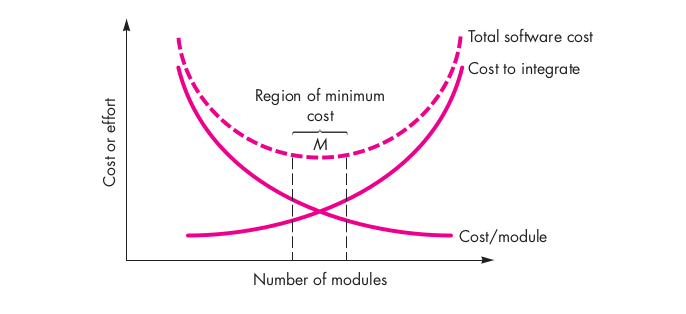
\includegraphics[width=0.8\textwidth]{figure_8_2.png}
	\caption{Đồ thị tương quan giữa số module và chi phí}
	\label{fig:fig8_2}
\end{figure}

Như đã thảo luận ở các phần trước, nếu bạn chia các vấn đề đủ nhỏ thì chi phí sẽ không đáng kể, nhưng điều này thực tế là không thể!! Ở\autoref{fig:fig8_2}thì nỗ lực chia nhỏ phần mềm thành các module riêng rẻ sẽ làm số lượng module tăng theo. Với một tập yêu cầu, số lượng module nhiều lên tương đương việc kích thước module riêng lẻ sẽ nhỏ hơn, chi phí phát triển modul sẽ ít đi. Tuy nhiên, khi số lượng module tăng lên, nỗ lực kết hợp chúng thành hệ thống sẽ tăng. Nhưng đặc điểm này sẽ dẫn đến đường cong ở\autoref{fig:fig8_2}. Như vậy, nếu có M module thì kết quả sẽ đạt được chi phí tối thiểu, nhưng không đủ chính xác để để xác định giá trị M. Đường cong đưa ra ở\autoref{fig:fig8_2}hữu ích khi xét đến tính module của phần mềm. Bạn nên module hóa, nhưng nên ở trong cùng lân cận của M (Region of minimum cost). Nên tránh các vùng undermodularity và overmodularity. Nhưng làm thế nào để xác định được vùng lân cận của M? Số lượng module nên là bao nhiêu? Những câu hỏi này đòi hỏi khả năng hiểu của các khái niệm khác của chương này.


Bạn nên module hóa thiết kế(và chương trình đích) sẽ giúp lập trình viên dễ lên kế hoạch, chi phí phần mềm có thể xác định và phân phối, những thay đổi có thể dễ dàng xác định, kiểm thử và tìm lỗi sẽ hiệu quả hơn và lâu dài hơn là hệ thống được bảo trình liên tục mà không có các sự cố nghiêm trọng xảy ra.


\subsection{Che giấu thông tin (Data hiding)}
Khái niệm module hóa dẫn ta tới một câu hỏi: "Làm cách nào để có thể chia một phần mềm thành một tập các module tốt nhất?". Nguyên tắc che giấu thông tin cho rằng các module nên được "characterized by design decisions that (each) hides from each other". Nói cách khác, các module nên được thiết kế sao cho thông tin (thuật toán và dữ liệu) nằm trong module không thể được truy cập từ những module khác không cần đến thông tin đó.

Che giấu cho rằng việc module hóa hiệu quả có thể đạt được bằng cách định nghĩa một tập các module độc lập, giao tiếp với nhau bằng lượng thông tin tối thiểu cần thiết để thực hiện chức năng của phần mềm. Quá trình trừu tượng hóa sẽ giúp định nghĩa các thực thể của phần mềm. Che giấu thông tin định nghĩa và áp đặt giới hạn truy cập (access constraint) tới những chi tiết cụ thể của module.

Việc áp dụng nguyên lý che dấu thông tin cho các hệ thống modular mang lại lợi ích lớn nhất khi ta sửa đổi hệ thống trong quá trình kiểm thử và sau này là quá trình bảo trì. Vì dữ liệu và chi tiết thuật toán (procedural detail) của module được che giấu khỏi những phần khác của hệ thống, các lỗi xuất hiện khi sửa đổi sẽ khó lan ra những phần khác của hệ thống.


\subsection{Độc lập chức năng}
Khái niệm độc lập chức năng \iindex{độc lập chức năng} được phát triển từ khái niệm separation of concerns, module hóa, trừu tượng hóa và che giấu thông tin. Trong bài luận bất hủ về thiết kế phần mềm, Wirth \cite{Wir71} và Parnas \cite{Par72} chỉ ra những kĩ thuật để nâng cao tính độc lập của module. Một thời gian sau, công trình của Stevens, Myers và Constantine đã hoàn thiện khái niệm này.

Độc lập chức năng đạt được bằng việc phát triển các module với một chức năng duy nhất. Nói cách khác, bạn nên thiết kế phần mềm sao cho mỗi module xử lý một tập con các yêu cầu cụ thể và sở hữu một \acrshort{API} API đơn giản.  \textit{Vậy tại sao chức năng lại quan trọng?}

Phần mềm được module hóa hiệu quả (với các module độc lập) sẽ dễ dàng phát triển hơn. Vì chức năng có thể được chia nhỏ, đóng gói lại và \acrshort{API} được đơn giản hóa. Module độc lập sẽ dễ dàng bảo trì (và kiểm thử) hơn vì tác dụng phụ do thiết kế hoặc do sửa đổi code bị giới hạn, ngăn lỗi của một phần ảnh hưởng tới các phần khác. Module độc lập còn giúp việc tái sử dụng dễ dàng hơn. Tóm lại, độc lập tính năng là chìa khóa dẫn tới thiết kế tốt, và thiết kế tốt là chìa khóa dẫn tới một phần mềm chất lượng.

Tính độc lập được đánh giá bằng hai yếu tố định tính sau: tính cố kết (cohesion) và tính gắn nối (coupling). Tính cố kết là thước đo sức mạnh tương đối của một module. Tính gắn nối là thước đo sự phụ thuộc lẫn nhau tương đối giữa các module.

Tính cố kết là sự mở rộng tự nhiên của khái niệm độc lập chức năng mô tả trong phần 3.6. Một module có tính cố kết thực hiện duy nhất một chức năng và không cần tương tác nhiều với các thành phần khác của chương trình. Mặc dù bạn luôn cần cố gắng để đạt được tính cố kết chặt chẽ (độc lập tính năng), việc sở hữu một thành phần thực hiện nhiều chức năng thường là cần thiết. Tuy nhiên, ta nên tránh một thành phần thực hiện nhiều chức năng mà không liên quan đến nhau.

Tính gắn nối là thước đo mối tương tác lẫn nhau giữa các module trong cấu trúc phần mềm. Tính gắn nối phụ thuộc vào độ phức tạp giao diện giữa các module. Trong thiết kế phần mềm, bạn nên cố gắng làm cho tính gắn nối thấp nhất. Sự kết nối đơn giản giữa các module sẽ giúp phần mềm dễ hiểu hơn và tránh được "hiệu ứng gợn sóng" (ripple effect)  \cite{Ste74}, tức là việc lỗi xuất hiện ở một phần của chương trình lan ra toàn hệ thống.



\subsection{Làm mịn (Refinement)}
\textit{Làm mịn}\index{làm mịn} từng bước (Stepwise refinement) là phương pháp thiết kế từ trên xuống (top-down) được đưa ra bởi Niklaus Wirth \cite{Wir71}. Chương trình được phát triển bằng các mức làm mịn liên tiếp các chi tiết thủ tục. Một cấp bậc được phát triển bằng việc phân tách một phát biểu vĩ mô về chức năng theo từng bước cho tới khi ta có thể biểu đạt phát biểu đó bằng ngôn ngữ lập trình.

Làm mịn thực chất là quá trình làm rõ, phân tích. Bạn bắt đầu bằng một phát biểu (hoặc mô tả) về tính năng được định nghĩa chung chung, trừu tượng. Nghĩa là câu phát biểu chỉ mang tính tổng quát, chung chung; không cung cấp được thông tin về cơ chế hoạt động của chức năng đó. Sau đó, bạn phân tách phát biểu đó thành phát biểu cụ thể, chi tiết hơn sau từng bước làm mịn.

Trừu tượng và làm mịn là hai khái niệm bổ sung cho nhau. Trừu tượng cho phép bạn che giấu chi tiết cấp thấp bên trong với những người không cần biết đến nó. Làm mịn giúp bạn tìm ra các chi tiết cấp thấp trong quá trình thiết kế. Cả hai khái niệm cho phép bạn tạo nên một mô hình thiết kế hoàn chỉnh.
\subsection{Aspects}
Một tập mối quan tâm sẽ được phát hiện trong quá trình phân tích yêu cầu. Những mối quan tâm này “bao gồm: ca sử dụng, tính năng, cấu trúc dữ liệu, vấn đề chất lượng dịch vụ, giới hạn của tài sản trí tuệ, hợp đồng” \cite{AOS07}.  Trong trường hợp lý tưởng, một mô hình yêu cầu có thể được sắp xếp sao cho mỗi mối quan tâm được cô lập và có thể giải quyết một cách độc lập. Trong thực tế, một số mối quan tâm có thể bao trùm cả hệ thống và không thể dễ dàng chia tách ra để giải quyết.

Khi bắt đầu thiết kế, các yêu cầu được biểu diễn theo thiết kế module. Với hai yêu cầu A và B, yêu cầu A giao (crosscuts) với yêu cầu B "if a software decomposition [refinement] has been chosen in which B cannot be satisfied without taking A into account” \cites{Ros04}. 

Ví dụ, cân nhắc 2 yêu cầu cho dự án \textbf{SafeHomeAssured.com} WebApp. Yêu cầu A được mô tả qua ca sử dụng \textbf{ACS-DCV} được nhắc đến trong chương 6 của tài liệu chính thức. Việc làm mịn thiết kế sẽ tập trung vào những module cho phép "người dùng đã đăng ký" truy cập vào các video được quay bởi camera trong một khu vực. Yêu cầu B là một yêu cầu chung chung về bảo mật: "người dùng đã đăng ký" phải được xác nhận trước khi sử dụng \textbf{SafeHomeAssured.com}. Yêu cầu này áp dụng được cho toàn bộ chức năng dành cho "người dùng SafeHome đã đăng ký".  Trong quá trình làm mịn thiết kế, A* là thể hiện thiết kế của yêu cầu A, B* là thể hiện thiết kế của B. Như vậy, A* và B* là thể hiện của các yêu cầu, và B* giao A*.

Một khía cạnh (aspects) là thể hiện của mối quan tâm giao thoa (crosscutting concern). Như vậy, thể hiện thiết kế B* của yêu cầu: "người dùng đã đăng ký" phải được xác nhận trước khi sử dụng \textbf{SafeHomeAssured.com}, là một khía cạnh của phần mềm \textit{SafeHome} WebApp. Chúng ta cần phát hiện các khía cạnh của chương trình và giải quyết chúng một cách thích hợp trong quá trình làm mịn và module hóa. Trong trường hợp lý tưởng, một khía cạnh của phần mềm là một module độc lập, thay vì một phần code nhỏ được rải rác khắp các phần của chương trình. Để đạt được điều này, kiến trúc thiết kế nên hỗ trợ cơ chế định nghĩa một khía cạnh - một module cho phép giải quyết một mối quan tâm xuyên suốt toàn bộ những mối quan tâm mà nó giao với.
\subsection{Refactoring}
Refactoring là một kĩ thuật sắp xếp lại chương trình để làm đơn giản hóa thiết kế của một thành phần nhưng không làm thay đổi chức năng hay hành vi của nó. Fowler \cite{Fow00} định nghĩa refactoring như sau: "Refactoring là quá trình thay đổi phần mềm sao cho không ảnh hưởng tới hành vi/chức năng của code, nhưng làm tốt thêm cấu trúc bên trong của phần mềm."

Khi phần mềm được refactor, thiết kế hiện tại được kiểm tra để tìm kiếm những yếu tố thừa, không sử dụng, thuật toán không tối ưu, cấu trúc dữ liệu không phù hợp, hoặc bất kỳ sai lầm thiết kế nào mà có thể sửa chữa để giúp thiết kế phần mềm tốt hơn. Ví dụ, trong lần thiết kế đầu tiên, có thể xuất hiện một thành phần có tính cố kết thấp (thực hiện 3 chức năng ít liên quan tới nhau). Sau khi cân nhắc kỹ càng, bạn có thể quyết định chia thành phần này thành 3 thành phần khác nhau, thực hiện một chức năng độc lập và có tính cố kết cao. Kết quả sẽ là một phần mềm dễ dàng tích hợp, test và bảo trì.


\subsection{Object-Oriented Design Concepts}
\textit{Mô hình hướng đối tượng}\index{mô hình hướng đối tượng} là mô hình được sử dụng rộng rãi trong phát triển phần mềm hiện nay. Bạn đọc có thể tham khảo phụ lục 2 ở tài liệu chính thức nếu chưa nắm vững khái niệm về thiết kế phần mềm hướng đối tượng như class và object, tính kế thừa, messages và tính trừu tượng.
\subsection{Design Classes}

Mô hình yêu cầu định nghĩa một tập các \textit{lớp phân tích} (chương 6 của tài liệu chính thức). Mỗi lớp đặc tả một số thành phần của miền vấn đề, tập trung vào các khía cạnh vấn đề mà người dùng nhìn thấy. Mức trừu tượng của một lớp phân tích là tương đối cao.

Khi mô hình thiết kế tiến hóa, bạn sẽ định nghĩa một tập \textit{lớp thiết kế}. Lớp thiết kế sẽ cung cấp chi tiết cụ thể để thực hiện chức năng lớp phân tích, và tạo ra một kiến trúc phần mềm để cung cấp giải pháp. Lớp thiết kế được phân ra làm 5 loại, mỗi loại tượng trưng cho một tầng của kiến trúc thiết kế \cite{Amb01}: 
\begin{itemize}
	
	\item \textit{Lớp giao diện người dùng} định nghĩa toàn bộ phép trừu tượng cần thiết cho tương tác người-máy \acrshort{HCI}. Sự tương tác thường được thể hiện qua một phép ẩn dụ (form đặt hàng, máy fax, …), và giao diện của lớp thiết kế có thể được phát triển từ phép ẩn dụ đó.
	\item \textit{Business domain classes} là kết quả của quá trình làm mịn lớp phân tích. Lớp này sẽ liệt kê những thuộc tính và service cần thiết để thực hiện chức năng thuộc miền kinh doanh (business domain).
	\item \textit{Process classes} thực hiện các business abstractions cấp thấp để quản lý business domain class.
	\item \textit{Persistent classes} đại diện cho các cơ sở lưu trữ dữ liệu (ví dụ như database) tồn tại độc lập với phần mềm.
	\item \textit{Lớp hệ thống} thực hiện chức năng quản lý và điều khiển phần mềm, cho phép hệ thống hoạt động, giao tiếp với môi trường tính toán và với thế giới bên ngoài.
\end{itemize}

Trong quá trình hoàn thiện kiến trúc phần mềm, mức trừu tượng sẽ được giảm do các lớp phân tích được chuyển thành thể hiện thiết kế. Nghĩa là, lớp phân tích thể hiện các đối tượng dữ liệu (và service liên quan được chúng sử dụng) ở mức độ chung chung. Lớp thiết kế thể hiện các chi tiết mang tính kỹ thuật cao, với mục đích hướng dẫn thực hiện chức năng.

Arlow và Neustadt \cite{Arl02} đề xuất rằng mỗi lớp thiết kế nên được review để đảm bảo tính hoàn thiện. Họ định nghĩa một lớp thiết kế hoàn thiện có 4 yếu tố sau:

\begin{description}
	\item[Đầy đủ và toàn diện.]  Một lớp thiết kế nên đóng gói đầy đủ thuộc tính và phương thức [...]. Ví dụ, lớp \textbf{Scene} cho một phần mềm chỉnh sửa video chỉ đầy đủ khi lớp đó chứa toàn bộ thuộc tính và phương thức gắn liền với công việc tạo video scene. Đảm bảo rằng lớp thiết kế chỉ nên chứa vừa đủ những phương thức để đạt được mục tiêu của lớp, không hơn không kém.
	\item[Tính nguyên thủy.] Phương thức của lớp thiết kế chỉ nên tập trung hoàn thành một tính năng (service) cho lớp. Service chỉ nên được thực hiện bằng duy nhất 1 phương thức. Ví dụ, lớp \textbf{VideoClip} cho phần mềm chỉnh sửa video có thể chứa thuộc tính \textbf{start-point} (điểm bắt đầu) và \textbf{end-point} (điểm kết thúc) để biểu diễn điểm bắt đầu và kết thúc của một clip. Phương thức \textit{setStartPoint()} và \textit{setEndPoint()} nên là phương tiện duy nhất để cài đặt giá trị cho điểm bắt đầu và kết thúc của clip.
	\item [Tính cố kết cao.] Một lớp thiết kế có tính cố kết cao sẽ chứa một tập hợp trách nhiệm duy nhất và các thuộc tính, phương thức để thực hiện trách nhiệm đó. Ví dụ, lớp \textbf{VideoClip} có thể chứa một tập hợp các phương thức để chỉnh sửa video. Miễn là mỗi phương thức tập trung duy nhất vào tính chất gắn liền với video clip, tính cố kết sẽ được đảm bảo.
	\item[Low coupling.]  Trong mô hình thiết kế, các lớp thiết kế luôn cần hợp tác với nhau, tuy nhiên nên hợp tác ở mức tối thiểu. Nếu một lớp thiết kế mang tính \textit{highly coupled} (nhiều lớp thiết kế hợp tác với nhau), hệ thống có thể khó thực hiện, kiểm thử và bảo trì. Nói chung, một lớp thiết kế trong một hệ thống con nên có ít thông tin về các lớp còn lại. Giới hạn này, được gọi với tên Law of Demeter \cite{Lie03} (nguyên lý hiểu biết ít nhất), cho rằng một phương thức chỉ nên giao tiếp với các lớp hàng xóm của nó.
\end{description}





